% 2007 年浙江卷理科第 20 题：直线 y=kx+b 与椭圆 x^2/4+y^2=1 交于 A、B，
%   记三角形 AOB 的面积为 S。
% 来源 PDF：gaokaomath-src/普通高考/2007/2007浙江理.pdf
% SHA-256：31c1d0d79ba11a3644a27b5ee3781f52caaf831209e8da63ddd8d7019cd06995
% 原页：2007浙江理.pdf 第 2 页（A3 三栏）第 2 栏，书页码 418。
% 重绘依据：按原页椭圆、割线与 A、B、O 的位置重绘。
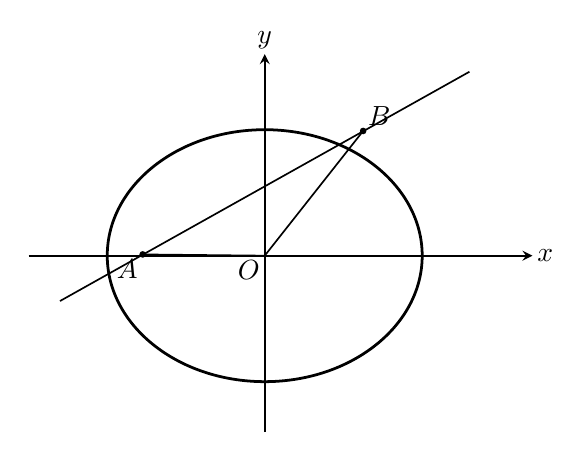
\begin{tikzpicture}[x=1.0cm, y=1.6cm, semithick,
  every node/.style={inner sep=1.5pt}]

  \draw[->,>=stealth] (-3.0,0) -- (3.4,0) node[right] {$x$};
  \draw[->,>=stealth] (0,-1.4) -- (0,1.6) node[above] {$y$};
  \node[below left] at (0,0) {$O$};

  % 椭圆 x^2/4+y^2=1
  \draw[line width=1pt] (0,0) ellipse (2 and 1);

  % 割线 y = 0.35x + 0.55（示意）
  \draw (-2.6,-0.36) -- (2.6,1.46);
  \coordinate (A) at (-1.55,0.01);
  \coordinate (B) at (1.25,0.99);
  \fill (A) circle (1.2pt);
  \fill (B) circle (1.2pt);
  \node[below left] at (A) {$A$};
  \node[above right] at (B) {$B$};

  \draw (A) -- (0,0) -- (B);
\end{tikzpicture}
